%%%%%%%%%%%%%%%%%%%%%%%%%%%%%%%%%%%%%%%%%
% Senior Thesis Poster Template
% Union College, Computer Science
%
% Author: Matthew Anderson (andersm2@union.edu)
% Version: Spring 2019.
%
% Initially Based on:
%    Jacobs Landscape Poster
%    LaTeX Template
%    Version 1.1 (14/06/14)
%
%    Created by:
%    Computational Physics and Biophysics Group, Jacobs University
%    https://teamwork.jacobs-university.de:8443/confluence/display/CoPandBiG/LaTeX+Poster
% 
%    Further modified by:
%    Nathaniel Johnston (nathaniel@njohnston.ca)
%
%    License:
%    CC BY-NC-SA 3.0 (http://creativecommons.org/licenses/by-nc-sa/3.0/)
%
%%%%%%%%%%%%%%%%%%%%%%%%%%%%%%%%%%%%%%%%%

\documentclass[final]{beamer}
\usepackage{tikz}
\usetikzlibrary{positioning}
% Debug mode
%\documentclass[debug]{beamer}
%\beamertemplategridbackground[.5in]

\usepackage[scale=1.11]{beamerposter} % Use the beamerposter package for laying out the poster

\usetheme{confposter} % Use the confposter theme supplied with this template

% Set color scheme for objects in poster.
\setbeamercolor{block title}{fg=jblue,bg=white} % Colors of the block titles
\setbeamercolor{block body}{fg=black,bg=white} % Colors of the body of blocks
\setbeamercolor{block alerted title}{fg=white,bg=unionred!100} % Colors of the highlighted block titles
\setbeamercolor{block alerted body}{fg=black,bg=unionred!10} % Colors of the body of highlighted blocks
% Many more colors are available for use in beamerthemeconfposter.sty

%-----------------------------------------------------------
% Define the column widths and overall poster size
% To set effective sepwid, onecolwid and twocolwid values, first
% choose how many columns you want and how much separation you want
% between columns
% In this template, the separation width chosen is 0.024 of the paper
% width and a 4-column layout onecolwid should therefore be (1-(# of
% columns+1)*sepwid)/# of columns e.g. (1-(4+1)*0.024)/4 = 0.22
% Set twocolwid to be (2*onecolwid)+sepwid = 0.464
% Set threecolwid to be (3*onecolwid)+2*sepwid = 0.708

\newlength{\sepwid}
\newlength{\onecolwid}
\newlength{\twocolwid}
\newlength{\threecolwid}
\setlength{\paperwidth}{46.8in} % A0 width: 46.8in
\setlength{\paperheight}{33.1in} % A0 height: 33.1in
\setlength{\sepwid}{0.024\paperwidth} % Separation width (white space) between columns
\setlength{\onecolwid}{0.22\paperwidth} % Width of one column
\setlength{\twocolwid}{0.464\paperwidth} % Width of two columns
\setlength{\threecolwid}{0.708\paperwidth} % Width of three columns
\setlength{\topmargin}{-0.5in} % Reduce the top margin size

\setlength{\belowcaptionskip}{1.5ex} % White space under figures
\setlength\belowdisplayshortskip{1.5ex} % White space under equations

\addtobeamertemplate{block end}{}{\vspace*{1.5ex}} % White space under blocks
\addtobeamertemplate{block alerted end}{}{\vspace*{1.5ex}} % White space under highlighted (alert) blocks
%-----------------------------------------------------------
\usepackage[dvipsnames]{xcolor}

\definecolor{blue}{RGB}{99,136, 180}
\definecolor{orange}{RGB}{255, 174, 52}
\definecolor{green}{RGB}{44, 160,44}
\definecolor{red}{RGB}{198, 39, 40}
\definecolor{purple}{RGB}{148, 103,189}
\definecolor{brown}{RGB}{140,86, 75}
\definecolor{pink}{RGB}{227 ,119 ,194}
\definecolor{gray}{RGB}{127, 127 ,127}



%----------------------------------------------------------------------------------------
%	TITLE SECTION 
%----------------------------------------------------------------------------------------

\title{Performance Evaluation of Maximum Matching Algorithm Implementations} % Poster title

\author{Jeremy Perez \and Janak Subedi} % Author(s)

\institute{Computer Science Department, Union College} % Institution(s)

%----------------------------------------------------------------------------------------

\begin{document}

% \begin{frame}[t] % The whole poster is enclosed in one beamer frame
  
  \begin{columns}[t]
    
    %\begin{column}{\sepwid}\end{column} % Empty spacer column

    % =============================================================
    % Column One
    % =============================================================
    
    \begin{column}{\onecolwid} % The first column
      
      
      % =============================================================
      % Abstract
      % =============================================================      
      
      % \begin{alertblock}{Abstract}
      %   \noindent \LaTeX{} is awesome!  You should definitely use it
      %   to make your poster.  In principle, anything that you could do
      %   in an article typeset in \LaTeX{} you could also do in a
      %   poster.  This template contains examples of how display
      %   various types of content on a \LaTeX{} poster.  This template
      %   only serves a suggestion about how to organize and present
      %   your research using \LaTeX{}.  This poster has more words than
      %   yours should.
        
      %   This maybe the only section of your poster that your viewer
      %   remembers, so make it count.
        
      % \end{alertblock}


      \begin{alertblock}{Question}
        
        \noindent How do variations in graph structure impact the efficiency of implementations of Maximum Matching algorithms?
        
      \end{alertblock}

      % =============================================================
      % Introduction
      % =============================================================
      
      \begin{block}{Introduction}
        \noindent The maximum matching problem is a theoretical computational problem focused on finding the largest set of edges in a graph where no two edges share a vertex. 

        The complexity of the max matching problem varies significantly based on the type of graph. The classes of approaches likewise are significantly different.

        \begin{itemize}
            \item  For \textbf{bipartite graphs} ($d = 2$), the problem is solvable in polynomial time.

            \begin{figure}[ht]

            \begin{tikzpicture}[scale=1.5]
                % Draw nodes for set U
                \node[circle, draw] (u1) at (0, 2) {1};
                \node[circle, draw] (u2) at (0, 0) {2};
                \node[circle, draw] (u3) at (0, -2) {3};
            
                % Draw nodes for set V
                \node[circle, draw] (v1) at (4, 2) {4};
                \node[circle, draw] (v2) at (4, 0) {5};
                \node[circle, draw] (v3) at (4, -2) {6};
            
                % Draw all edges (undirected)
                \draw[thick] (u1) -- (v1); % Edge between 1 and 4
                \draw[thick] (u1) -- (v2); % Edge between 1 and 5
                \draw[thick] (u2) -- (v1); % Edge between 2 and 4
                \draw[thick] (u2) -- (v3); % Edge between 2 and 6
                \draw[thick] (u3) -- (v2); % Edge between 3 and 5
                \draw[thick] (u3) -- (v3); % Edge between 3 and 6
            
                % Highlight the matching edges
                \draw[thick] (u1) -- (v1); % Highlight matching edge between 1 and 4
                \draw[thick] (u2) -- (v3); % Highlight matching edge between 2 and 6
                \draw[thick] (u3) -- (v2); % Highlight matching edge between 3 and 5
            \end{tikzpicture}
             \caption{A bipartite graph with maximum matching of 3}
            \end{figure}

            \item  For \textbf{$d$-partite graphs} ($d > 2$), the problem becomes NP-hard, requiring more complex and often approximate methods.
            \begin{figure}[ht]
            \centering
            \begin{tikzpicture}[scale=1, transform shape]
                % Nodes
                \node[draw, circle] (v1) at (0, 9) {$v_1$};   
                \node[draw, circle] (v2) at (0, 6) {$v_2$};
                \node[draw, circle] (u1) at (3, 9) {$u_1$};   
                \node[draw, circle] (u2) at (3, 6) {$u_2$};
                \node[draw, circle] (w1) at (6, 9) {$w_1$};   
                \node[draw, circle] (w2) at (6, 6) {$w_2$};
            
                % Edges
                \draw[red, thick] (v1) -- (u2);   % Matching edge
                \draw[orange, thick] (v2) -- (u2);
                \draw[green, thick] (v2) -- (u1);  % Matching edge
                \draw[green, thick] (u1) -- (w1); % Matching edge
            
                \draw[orange, thick] (u2) -- (w1); % Matching edge
                \draw[red, thick] (u2) -- (w2);    % Non-matching edge
            \end{tikzpicture}
            \caption{A tripartite graph with maximum matching of 2}
            \label{fig:tripartite_graph}
            \end{figure}
        \end{itemize}
        
        \noindent Classes of algorithms which we've implemented include

        \begin{itemize}
            \item Greedy Algorithms
            \item Tree Traversal Algorithms
            \item Heuristic Algorithms
            \item Approximation Algorithms
            \item Network Flow Algorithms
            \item Integer Programming Algorithms
        \end{itemize}
        



    \end{block}
      

      
    \end{column}
    
    %\begin{column}{\sepwid}\end{column} % Empty spacer column

    % =============================================================
    % Column Two
    % =============================================================
    
    \begin{column}{\onecolwid} 
      

      % =============================================================
      % Methods
      % =============================================================
      
      \begin{block}{Methods}
        \noindent
        We focus on developing \textbf{courses}, which are specialized test sets, meant to highlight an algorithm's dependence on a feature of the graph. 

        We then performed a series of performance evaluations by \textbf{racing} every algorithm across a series of these courses and assessing each algorithm’s accuracy, and run time on these courses. We hope to capture performance disparities between each algorithm.        
        
      \end{block}

      \begin{block}{Races and Courses}        
      \noindent
        Each course was developed to emphasize different graph characteristics based on the following properties:
        \begin{itemize}
            \item $d$: the number of partitions in the graph,
            \item $n$: the number of vertices,
            \item $m$: the number of edges, and
            \item $E$: the set of edges.
        \end{itemize}
        By treating all possible graph configurations as a set $A$, any subset $C\subseteq A$ can represent a course. Since $A = C \cup C^C$, we made sure to include the complement sets as additional courses. Some examples of courses we have studied are:
        \begin{enumerate}
        \item Perfect Matching ($n=m$)
        \item Non-Perfect Matching ($n!=m$)
        \item Large Vertex Count ($n>1000$)
        \item Dense Graphs ($m > \frac{n^d}{2}$)
        \item Sparse Graphs ($m << \frac{n^d}{2}$)
        \end{enumerate}
      
        % \noindent Here you should outline your approach for answering your research
        % question.  While this can be handled in prose, it can be done more
        % effectively as

      \end{block}
      \begin{block}{Performance Metrics}


      
      \noindent For a given solver, let $C$ denote the set of test cases in a course. Let $S\subseteq C$ denote the set of solved test cases. For any test case $e\in C$, let $t_e$ denote the time taken to complete a test case in seconds.
      
      \begin{itemize}
        \item \textbf{Accuracy} measures the number of cases correctly solved over the total number of cases with timeouts.
      
        \item  The \textbf{Total Time} (TT) metric is the total time taken to solve an entire course. 
          \[TT = \sum_{e\in S} t_e\]
          
          
        % \item   The \textbf{PAR-2} metric commonly utilized in SAT Competitions is used to evaluate the performance of solvers with respect to time taken to complete a course and the number of timeouts incurred by the solver.
        %   \[PAR2 = TT + 2L| C \backslash S|\]
      \end{itemize}



        
      \end{block}
      
    \end{column}
    
    %\begin{column}{\sepwid}\end{column} % Empty spacer column

    % =============================================================
    % Column Three
    % =============================================================
    
    \begin{column}{\onecolwid}
      
      
      % =============================================================
      % Results
      % =============================================================
      
      \begin{block}{Results for Bipartite Solvers}
        
        % \noindent Here you describe the results of following your
        % methodology.  In CSC 498, you may only have preliminary
        % results, discuss that here.  You might talk about difficulties
        % encountered while following your method.  It should be clear
        % from this section and the methods section what you actually
        % did.  Tables and graphs are appropriate here.  Make sure to
        % title, label axes, and give units where necessary.

        \begin{table}
        \centering
        \begin{tabular}{| l| c | c | c | c |}
        \toprule
         &
        \multicolumn{4}{|c|}{\textbf{Courses With 1s Timeout}}    \\
        \multicolumn{1}{|C|}{\textbf{Solver}} &
        \multicolumn{2}{|c|}{\textbf{N > 1000}} & \multicolumn{2}{|c|}{\textbf{Non-Perfect}}\\
        \midrule
        {}   & TT (s)   & ACC (\%) &TT (s)  & ACC(\%)\\
        \textcolor{red}{\textbullet}Vinh-Hopcroft-K   & 1     & 100  &  7& 100\\
        \textcolor{brown}{\textbullet}Kurtik-Hopcroft-K   &  2 &  100 &  7 & 100\\
        \textcolor{green}{\textbullet}Vinh-Edmond-K &  2    &  100 &  8 & 100\\
        \textcolor{orange}{\textbullet}EthanO-Hopcroft-K   &  11 &  100&  54 &  100\\
        \textcolor{blue}{\textbullet}Jacob-PULP-IP   & 12& 100 &  35 & 100\\
        \textcolor{gray}{\textbullet}Kurtik-Ford-Fulkerson   &  21 &  100&  28 & 100\\
        \textcolor{pink}{\textbullet}Huyen-Edmonds-K   & 80& 19.1 &  90 & 84.1\\
        \textcolor{purple}{\textbullet}Jeremy-GPT-Approx   &  89 &  0 &  261 &  70.86\\

        \bottomrule
        \end{tabular}
        % \caption{Comparison of percentages.}

        \end{table}

        
        % \vspace{-2ex}
        \begin{figure}[h]
          \begin{center}
            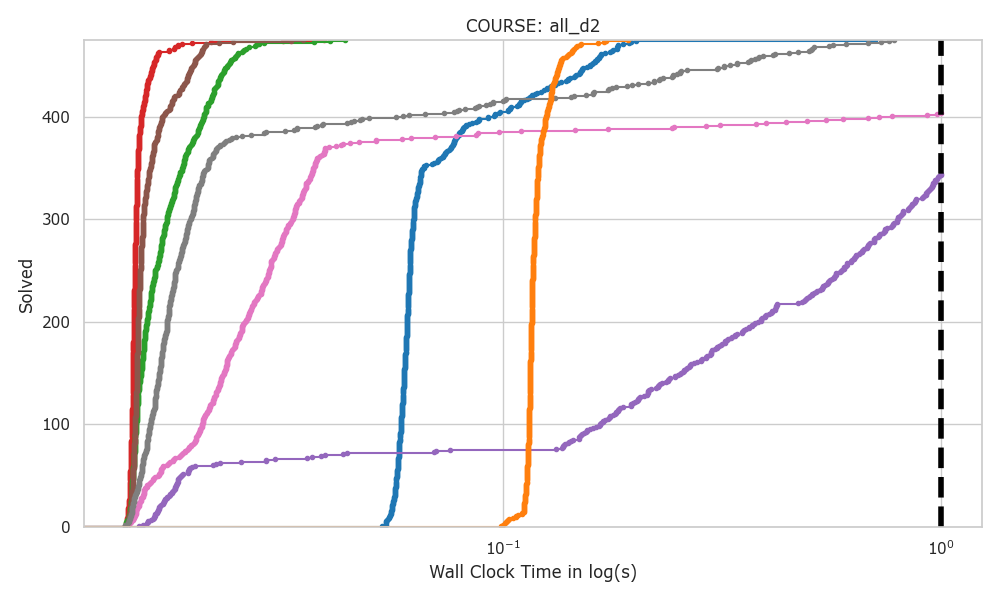
\includegraphics[width=1\linewidth]{figs/d2/all_d2.png}

            \caption{Performance of d2 Solvers against all test with a 1 second timeout}
          \end{center}
        \end{figure}

      \noindent With a 1 second timeout, some algorithms performed fairly bad, for instance, the GPT-Approximation algorithm was not able to complete a single large graph instance for graph's with more than $1000$ vertices. This clearly showcases that the algorithm is really bad at handling large graphs where as, an algorithm like Hopcroft Karp performed fairly well. This framework succeeds at effectively comparing algorithms runtimes as intended. 

      By varying the runtime between implementations of the same algorithm, we can visualize just how efficient they are with respect to each other. 

      Our preliminary results indicate that Hopcroft-Karp remains to be the fastest algorithm for Bipartite problems. 
      
      This seems to work as an informal runtime analysis.

        
      \end{block}


      % =============================================================
      % Analysis
      % =============================================================
      
      % \begin{block}{Analysis}

        
      %   % This isn't the only way to typeset algorithms, you can also use
      %   % the algorithmic, algorithms packages, or the codebox environment
      %   % provided by the textbook in CSC 250.
        
      %   % \begin{figure}[h]
      %   %   \IncMargin{1.25em}
          
      %     % \begin{algorithm}[H]
            
      %     %   \SetKwInOut{Input}{Input}\SetKwInOut{Output}{Output}
      %     %   \Input{$\delta \ge 0$, indicating the quality of poster
      %     %     required (larger is better).}
            
      %     %   \Output{A string containing the \LaTeX{} source of a poster
      %     %     with quality at least $\delta$.}
            
      %     %   $poster = ""$\;
      %     %   \While{$\proc{Quality}(poster) < \delta$}{
      %     %     $poster = \proc{Revise}(poster)$\;
      %     %     Run \texttt{make}\;
      %     %     \While{$\proc{CompileError}(poster)$}{
      %     %       Decrement $poster$\;
      %     %       Run \texttt{make}\;
      %     %     }
      %     %   }
      %     %   \Return $poster$\;
            
      %     % \end{algorithm}
      %   %   \DecMargin{1.25em}
      %   %   \caption{Algorithm for making \LaTeX{} posters. Warning: This
      %   %     algorithm may not halt!}
      %   % \end{figure}
      %   \medskip
  
        
      % \end{block}
      
    \end{column} 
    
    %\begin{column}{\sepwid}\end{column} % Empty spacer column


    % =============================================================
    % Column Four
    % =============================================================
    
    \begin{column}{\onecolwid} 

      % =============================================================
      % Conclusions
      % =============================================================

      \begin{block}{Results for Hypergraph Solvers}

              \begin{table}
        \centering
        \begin{tabular}{| l| c | c | c | c |}
        \toprule
        &
        \multicolumn{4}{|c|}{\textbf{Courses With 5m Timeout}}\\
        \multicolumn{1}{|C|}{\textbf{Solver}} &
        \multicolumn{2}{|c|}{\textbf{Random}} & \multicolumn{2}{|c|}{\textbf{Non-Perfect}}\\
        \midrule
        {}   & TT (s)   & ACC (\%) &TT (s)  & ACC(\%)\\
        \textcolor{blue}{\textbullet}Janak-BruteForce   & 148 &  79.6&  40 & 18.68\\
        \textcolor{red}{\textbullet}Jeremy-A*   &  655& 11.66 &  10 & 86.81\\
        \textcolor{green}{\textbullet}Jacob-PULP-IP   &  938&  99.17&  646 & 96.70 \\
        \textcolor{orange}{\textbullet}Jeremy-CPLEX-IP   &  60&  87.10&   60& 13.19\\
        \textcolor{purple}{\textbullet}Jeremy-Greedy   &  2&  3.03&  2 & 9.89\\

        \bottomrule
        \end{tabular}
        % \caption{Comparison of percentages.}

        \end{table}
        \begin{figure}[h]
          \begin{center}
            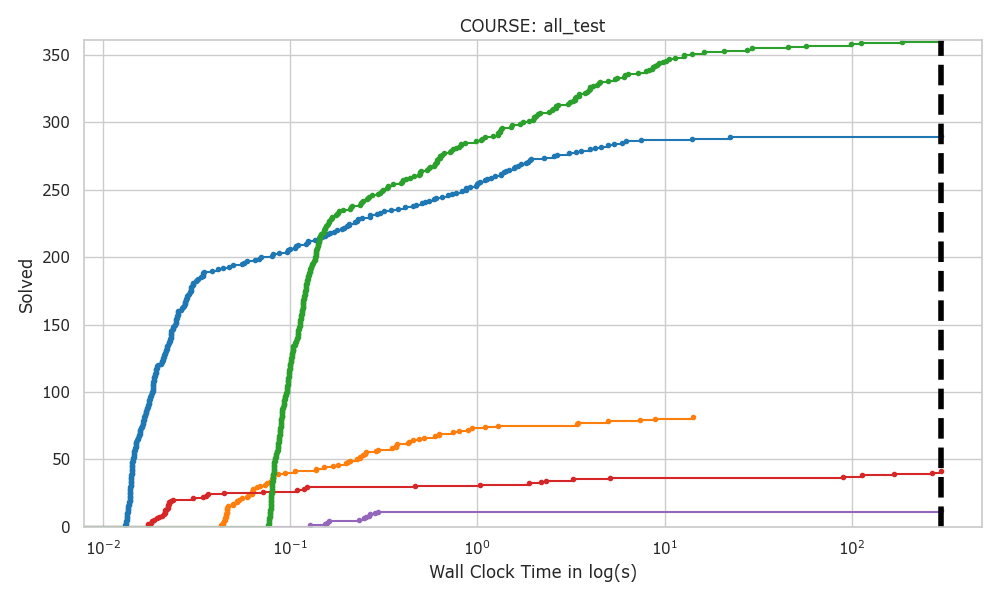
\includegraphics[width=1\linewidth]{figs/d/all_test.png}

            \caption{Performance of d-partite Solvers against all tests with a 5-minute timeout.}
            \end{center}
        \end{figure}
      \end{block}

      
      \begin{block}{Conclusions}

        After seeing great disparities in performance in d-partite algorithms, understanding how we've partitioned the solution space and how algorithms traverse into it, we find this to be an effective model for partitioning all possible graph configurations.
        
        % We believe that it is possible to make a combined algorithm that in general performs well particularly for each graph characteristic we focused on.
      
        
        % \noindent Here you describe what conclusions the audience should
        % reach from your analysis.  Did you answer your research question?
        % Discuss any threats to validity in your method, data, or analysis,
        % or any assumptions that were important to reach your conclusions.
        % What would you do differently if you could do it again, or work on
        % this project for another term (or in graduate school)?  For example,
        % I'd like to add a \texttt{tikz} example to this poster like the one
        % below.
        
        % \begin{center} % Centers the diagram on the page.
          % Making a diagram using the specified style parameters.
        %   \begin{tikzpicture}[->,>=stealth',shorten >=1pt,auto,node distance=10cm,
        %       thick,line width=1mm]
        %     \tikzstyle{every state}=[fill=white,draw=black,text=black]
            
        %     % Set the states.
        %     \node[initial,state] (q1)               {$q_1$};
        %     \node[state]                   (q2) [right of=q1] {$q_2$};
        %     \node[state]                   (q3) [below of=q1] {$q_3$};
        %     \node[state,accepting]         (q4) [right of=q3] {$q_4$};
            
        %     % Set the transitions. 
        %     % Syntax: (<start node>) edge [edge modifier] node [node modifier] {<edge label>} (<end node>)
        %     \path 
        %     (q1) edge [loop above] node {0} (q1)
        %     edge [bend left]  node {1,$\varepsilon$} (q2)
        %     (q2) edge              node {0} (q3)
        %     edge [bend left]  node {1} (q1)
        %     (q3) edge              node {0} (q1)
        %     edge              node [below] {1} (q4)
        %     (q4) edge [loop right] node {0,1} (q4);   % This semi-colon must be here.
        %   \end{tikzpicture}
        % \end{center}
        
        
      \end{block}

      % =============================================================
      % Acknowledgements
      % =============================================================

      \vfill
      
      % \begin{block}{Acknowledgments}
        
      %   \noindent This section is optional.  Here you should thank
      %   anyone other than your advisor that provided help to you in
      %   your project.  This can be other students, faculty, or staff.
      %   If you received an SRG to complete your project that should be
      %   mentioned here.
        
      %   For example, I'd like to thank my colleagues for giving me
      %   feedback on my drafts of this poster template, and David Frey
      %   for making sure it will print appropriately.
        
      % \end{block}

      % =============================================================
      % References
      % =============================================================
      
      % \begin{block}{References}
      %   \nocite{*} 
      %   % \small{\bibliographystyle{acm}
      %   %   \bibliography{poster}\vspace{0.75in}}
      % \end{block}
\begin{block}{References}
  \scriptsize % Reduces the font size even more
  \setlength{\parindent}{0pt} % No indentation
  \setlength{\parskip}{0pt} % No extra spacing between paragraphs
  \setlength{\itemsep}{0pt plus 0.2ex} % Further reduces space between items

  \begin{thebibliography}{9}

    \bibitem{hopcroftkarp}
    Hopcroft, J. E., \& Karp, R. M. (1973). An \(n^{5/2}\) Algorithm for Maximum Matchings in Bipartite Graphs. \textit{SIAM Journal on Computing}, 2(4), 225-231. doi:10.1137/0202019.

    \bibitem{edmondskarp}
    Edmonds, J., \& Karp, R. M. (1972). Theoretical Improvements in Algorithmic Efficiency for Network Flow Problems. \textit{J. ACM}, 19(2), 248-264. doi:10.1145/321694.321699.

    \bibitem{fordfulkerson}
    Ford, L. R., \& Fulkerson, D. R. (1956). Maximal Flow Through a Network. \textit{Canadian Journal of Mathematics}, 8, 399-404. doi:10.4153/CJM-1956-045-5.

    \bibitem{pulp}
    Mitchell, S. D., \& Roy, J. (2023). PuLP: A Python Library for Linear Optimization. Available at: \url{https://coin-or.github.io/pulp/}. Accessed: 2023-11-05.

    \bibitem{cplex}
    IBM ILOG CPLEX. (2023). CPLEX Optimizer. Available at: \url{https://www.ibm.com/products/ilog-cplex-optimization-studio}. Accessed: 2023-11-05.

  \end{thebibliography}
\end{block}





    \end{column} 
    
  \end{columns}
  
% \end{frame}

\end{document}
